\documentclass{article}
\usepackage[utf8]{inputenc}
\usepackage{graphicx}

\begin{document}


Cities produce large amounts of spatio-temporal data from several domains, like traffic, air quality, crime events, epidemic outbreaks, and social media, among many others. This data can help cities and their communities to develop innovative solutions to pressing urban problems. However, one challenge is the integration and harmonization of data from different sources and different types. One example of this is the geolocated data, which might be at exact locations or aggregated at different spatial levels like neighborhoods and municipalities.

To address this problem, it is possible to aggregate the features over the same space within areas such as neighborhoods or postal code zones. One inconvenient with this approach is that such zones might require updating as cities change and often their edges are defined arbitrarily, moreover, those areas have unusual shapes and sizes, making difficult a direct comparison among them. We used Ubers's H3 hexagonal hierarchical spatial indexing (H3) grid system \cite{uber2019} to generate spatially continuous hexagons. One example of the data at different spatial levels is shown in image \ref{fig:spatialLevels}. The H3 grid system was developed for ride pricing optimization, spatial data visualization, and data exploration. Data can be aggregated into hexagonal areas or cells at 16 different resolutions. Additionally, it has an indexing system that allows to group and searches for grouped data efficiently.

We aggregated geospatial data from different granularities to tackle two challenges in two Colombian cities, Bogotá and Cali. In the former city, we conducted a study about the impact of the spatio-temporal dynamics of Twitter posts on the sales of a fast-food chain of restaurants; in the latter city, we proposed models that help to understand the dynamics of the covid-19 outbreak locally. In both cases, we took into account demographic variables, e.g. the number of inhabitants, percentage of income, and the presence of places like hospitals, universities, and parks nearby.

\begin{figure}[ptb]
    \centering
    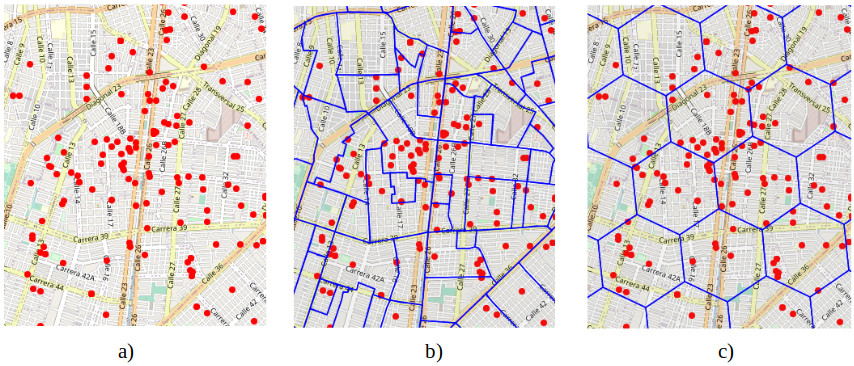
\includegraphics[width=.95\linewidth]{imgs/geolocations}
    \caption{Spatial data at different levels: a) exact location; b) data grouped by neighborhoods; and c) data grouped by hexagons.}
    \label{fig:spatialLevels}
\end{figure}

\bibliography{bibliografia} 
\bibliographystyle{ieeetr}
\end{document}